\section{Iterative Model Update}
In this section, we describe how we iteratively update a dirty model based on
a cleaned batch of data.
We will show that this model update procedure can be interpreted as a Stochastic 
Gradient Descent (SGD) algorithm, which gives us a theoretical framework to analyze
convergence and bound the error at each step.
This theoretical framework will also inform how we should 

\subsection{Model Update Problem}
Suppose we have a cleaned batch of data $S_{clean}$ with features and labels $(X_{clean},Y_{clean})$, and a dirty model $\theta^{(d)}$. 
In the model update problem, we update the dirty model with some function $f(\cdot)$ i.e.,:
\[
\theta^{new} \leftarrow f(X_{clean},Y_{clean},\theta^{(d)})
\]
Our goal is that these updates should minimize the error the updated model and the true model $\theta^{(c)}$ (if we cleaned and trained over the entire data):
\[
error(\theta^{new}) = \| \theta^{new} - \theta^{(c)} \|
\]

\subsection{Exploiting the Model's Geometry}
\sys addresses the update problem by using the model's geometry.
We restrict the class of Machine Learning models to convex regularized loss problems.
That is, as we vary the model $\theta$ the loss is bowl-shaped (visualized in Figure \ref{update-arch2}a).
The model update problem can be visualized as follows.
We have a model $\theta^{(d)}$ (visualized in red) that is suboptimal with respect to the clean data.
We want to get to the optimal clean model $\theta^{(c)}$ which is visualized as a yellow star.

\begin{figure}[ht!]
\centering
 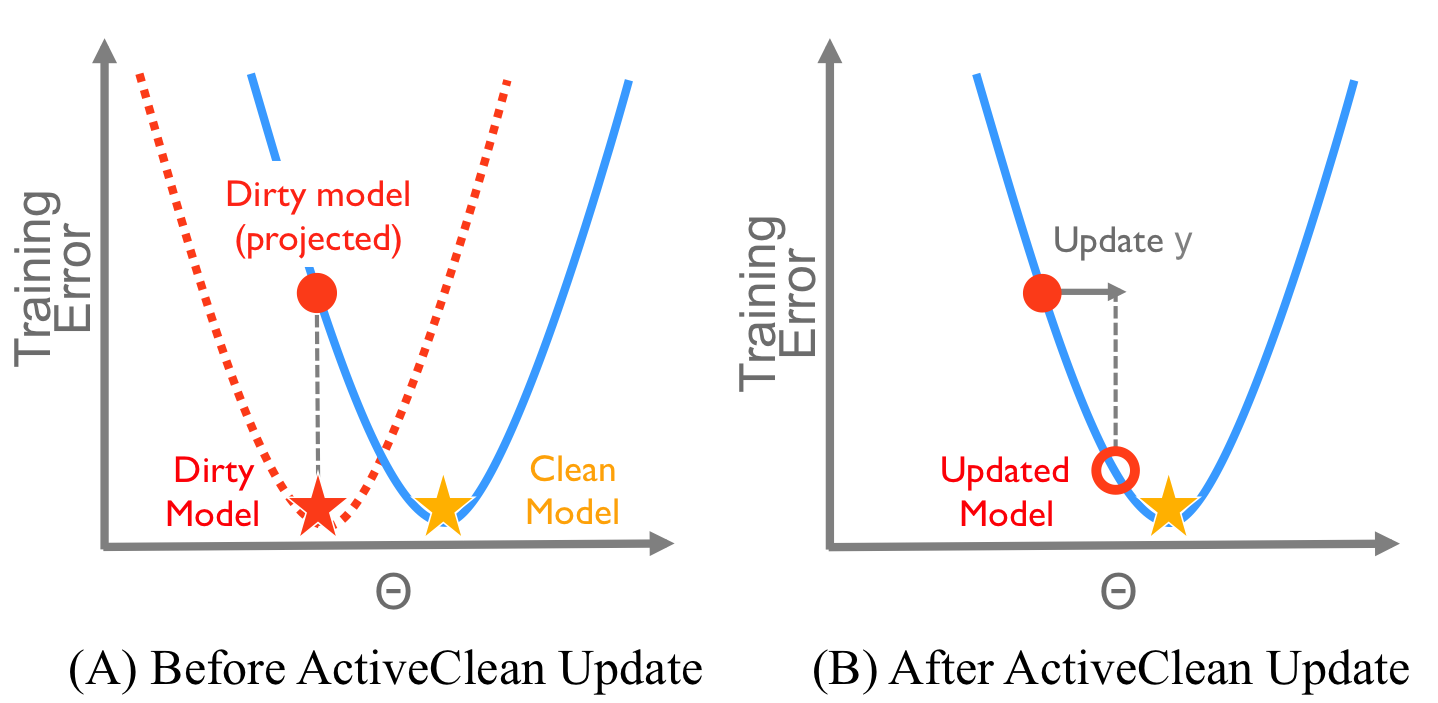
\includegraphics[width=\columnwidth]{figs/update-arch2.png}
 \caption{In \sys, we explore an important class of Machine Learning problems where the loss function (i.e., training error) varies convexly. A stale model can be thought of as a sub-optimal point and we want to move towards the optimal point. \label{update-arch2}}
\end{figure}

Ideally, we want an update that goes in the right direction (one that points to the optimum) along the loss curve (Figure \ref{update-arch2}b).
Mathematically, this direction corresponds to gradient of the loss with respect to $\theta$, and we need to move some distance $\gamma$ along this direction:
\[
\theta^{new} \leftarrow \theta^{(d)} - \gamma \cdot \nabla\phi(\theta^{(d)})
\]
However, since we can only clean a sample of data, we only approximate the globally optimal direction.
Our class of Machine Learning models are based on loss minimization, that is they are a sum of losses, and we know that sums commute with derivatives.

Let $S$ be a sample of data, where each $i \in S$ is drawn with probability $p_i$.
We can approximate the global gradient:
\[
\nabla\phi(\theta) \approx g_{S}(\theta) = \sum_{i \in S}\frac{1}{p_i}\nabla\phi(x_i^{clean},y_i^{clean},\theta)
\]
Then for every batch of data cleaned, we apply the update to the current best model estimate:
\[
\theta^{(t)} \leftarrow \theta^{(t-1)} - \gamma \cdot g_{S}(\theta^{(t-1)})
\]
In other words, we are moving approximately in the right direction.
The intuition, which we will formalize in Section \ref{sgd}, is that if we are on average in the right direction the algorithm is guaranteed to converge with analytics bounds on the convergence rate.
At the optimal point, the expected gradient will be zero.
So intuitively, this approach iteratively moves the model downhill, or corrects, the dirty model until the budget is reached.

The tricky part is that only a subset of the records of the records are dirty.
In our architecture, we suggested that we want to clean only the records that
are actually dirty $R_{dirty}$.
For example, as data are cleaned, there is no need to resample this data.
The consequence of this is that the estimate $g_{S}(\theta)$ is now biased.
We also have to compensate for this bias by averaging this estimate with the gradient with respect to the clean data:
\[
g_C(\theta) = \sum_{i \in R - R_{dirty}}\nabla\phi(x_i^{clean},y_i^{clean},\theta)
\]
Then, for weights $\alpha,\beta$ which we will subsequently discuss how to select:
\[
g(\theta) = \alpha \cdot g_C(\theta) + \beta \cdot g_S(\theta)
\]
So then our final gradient update becomes:
\[
\theta^{(t)} \leftarrow \theta^{(t-1)} - \gamma \cdot g(\theta) \blacksquare
\]

Here, we can draw an analogy to Materialized View maintenance, since after all, a model parameterized by $\theta$ is just a table of floating point numbers.
Krishnan et al. proposed a technique called sample view cleaning, in which they take a clean sample of data and propogate the updates to a Materialized View.
Similarly, in this work, we take the information from a sample of cleaned data and propagate an update with the gradient.
The insight that many mathematical problems are analogous to view maintenance has recently been noted others as well \cite{nikolic2014linview}.

\subsection{Iterative Model Correction Algorithm}
Following from this geometric analysis, we propose the iterative model correction algorithm.
We initialize the algorithm with $\theta^{(d)}$ which is the dirty model.
At each iteration $i=\{1,...,t\}$, we clean a batch of data $b$ selected from the set of candidate dirty records $R_{dirty}$.
Then, starting with $\theta^{(d)}$, we apply an averaged gradient update to get $\theta^{(i)}$.
We iterate until our budget of cleaning $k = t \cdot b$ record is reached.

We present the algorithm here:
\begin{enumerate}[noitemsep]
\item Initialize with $\theta^{(0)} = \theta^{(d)}$ as the dirty model, $t$ iterations, with a batch size $b$, $R_{dirty}$, and $R_{clean} = R - R_{dirty}$.
\item Hyperparamters $\gamma$, $\alpha$, $\beta$.
\item For rounds i=1...t
\begin{enumerate}
	\item Draw a sample of $b$ records from $R_{dirty}$ called $S_{dirty}$.
	\item Apply data cleaning to the sample of data call the result $S_{clean}$.
	\item Calculate the gradient over the sample of clean data and call the result $g_S(\theta^{(i-1)})$
	\item Calculate the average gradient over all the data in $R_{clean}$, and call the result $g_C(\theta^{(i-1)})$
	\item Apply the following update rule:
	\[
	\theta^{(i)} \leftarrow \theta^{(i-1)} - \lambda \cdot(\alpha\cdot g_S(\theta^{(i-1)}) + \beta \cdot  g_C(\theta^{(i-1)}))
	\]
	\item Update the sets $R_{dirty} = R_{dirty} - S_{dirty}$, $R_{clean} = R_{clean} \cup S_{clean}$
\end{enumerate}
\item Return $\theta^{(T)}$
\end{enumerate} 

\subsubsection{Selecting the Parameters}
The proposed update policy makes intuitive sense.
However, we have still have to set the parameters $\lambda$, $\alpha$, $\beta$.
We will show that theory from the stochastic optimization literature can allow us to understand this iterative algorithm.
First, we will review all of the parameters that need to be set.

\vspace{0.5em}

\noindent\textbf{Step Size $\gamma$ : } The first problem is that we have not explained how to pick the step size $\gamma$. In other words, how far should we travel in the gradient direction.

\vspace{0.5em}

\noindent\textbf{Step Size $\alpha,\beta$ : } The next problem is deriving the proportions with which we should combine $g_S(\theta)$ and $g_C(\theta)$. It turns out that $\alpha = \frac{R_{clean}}{R}$ and $\beta = \frac{R_{dirty}}{R}$, and we will show a derivation below.

\vspace{0.5em}

\noindent\textbf{Choosing $S$: } As we mentioned, the optimal clean model depends on \emph{all} the clean data, not just a sample. 
So $g_S$ is really an approximation of the gradient with some error $g^* \pm \epsilon$. 
The quality of the update depends on how well we can approximate $g^*$ using $g_S$.
The problem is how should we construct the sample of data to clean $S$ to get the most accurate update.
In particular, how should we choose the sampling probabilities $p_i$ for each $i \in S$ such that the error is minimized.

\subsubsection{Physical Design Considerations}
From a systems perspective, the important step in the update algorithm is step 3a.
We have to query a sample of candidate data points from $R_{dirty}$ which 
can be expensive.
As we clean data, we can maintain an index on which points are dirty and clean.

\subsection{Stochastic Gradient Descent}\label{sgd}
This update policy can be formalized as a class of very well studied algorithms called Stochastic Gradient Descent.
This gives us a theoretical framework to understand and analyze our update rule, bound the error, and choosing points to clean.
Mini-batch stochastic gradient descent (SGD) is an algorithm for finding the optimal value
of $\theta$, given the convex loss, and data.
In SGD, we start with an abitrary initialization and iterate to convergence.
In our case, we start with an initialization which is the dirty model, the model trained completely on the dirty data.
Then, at each iteration we sample a mini-batch of data on which we apply our expensive data cleaning operations.
The update rules in SGD mirror our update policy:
 \[
 \theta^{(t+1)}\leftarrow\theta^{(t)}-\gamma\frac{1}{\mid S^{(t)}\mid}\sum_{i\in S^{(t)}}\nabla\phi(x_i,y_i,\theta^{(t)})
 \]

\vspace{0.5em}

\noindent\textbf{ Setting $\gamma$: } There is extensive literature in machine learning for choosing $\gamma$ appropriately. $\gamma$ can be set either to be a constant or decayed over time. Many machine learning frameworks (e.g., MLLib, Sci-kit Learn, Vowpal Wabbit) automatically set learning rates or provide different learning scheduling frameworks. 
In our experiments, we use a technique called inverse scaling where there is a parameter $\gamma_0=0.1$, and at each iteration we reduce it to $\gamma_t = \frac{\gamma_0}{\mid S \mid t}$. 

\vspace{0.5em}

\noindent\textbf{ Convergence: } The next property of concern is convergence. Convergence properties of batch SGD formulations has been well studied \cite{dekel2012optimal}. 
The conditions on this convergence are essentially that at each step the estimate of the gradient $g_S$ has to be unbiased, that is on average correct. 

\begin{proposition}
For an appropriately chosen learning rate $\gamma_t$, batch stochastic gradient descent will converge if $\mathbb{E}(g_S)=g^*$.
\label{unbiased}
\end{proposition}

A direct result of convergence is a guarantee on statistical consistency.
Another interesting consequence of this result is that we can sample $S$ in any way that we want
as long as our estimate in unbiased.

\vspace{0.5em}

\noindent\textbf{ Convergence Rate: } The convergence rates of SGD are also well analyzed \cite{dekel2012optimal,bertsekas2011incremental,zhao2014stochastic}. 
Suppose, a user cleans a batch size of $b$ examples at each iteration.
This allows us to bound the error of intermediate models and understand the expected number of steps before a model within a certain error. 

\begin{proposition}
For a general convex loss, a batch size $b$, and $t$ iterations, the convergence rate is bounded by $O(\frac{\sigma^2}{\sqrt{bt}})$. 
$\sigma^2$ is the variance in the estimate of the gradient at each iteration:
\[
\mathbb{E}(\|g_S - g^*\|^2)
\]
\end{proposition}

There is an interesting tradeoff between batch size an convergence rate.
Increasing the batch size reduces the variance $\sigma^2$, however it does
mean at each iteration you are doing more work.
In a data cleaning context, this is a problem since the bottlneck is the work at 
each iteration not the number of iterations.

\subsubsection{Reducing the Variance $\sigma^2$}\label{dist-samp}
In the Machine Learning and Optimization literature, SGD algorithms are optimized to avoid scanning the entire data.
Uniform sampling is cheap so it is the preferred solution.
However, there are a few observations about the data cleaning problem that suggest that we can do better if we carefuly select which points to clean.
The key property that we need to preserve is unbiasedness (Proposition \ref{unbiased}).

\vspace{0.5em}

\noindent\textbf{Observation 1. Detection vs. Cleaning: } In many applications, enumerating the set of corrupted records is much easier than cleaning them. For example, we may be able to select the set of rows that have missing values but actually filling those missing values is expensive. Likewise, in the constraint literature, selecting a set of rows that have a violated constraint can be done in polynomial time, however, fixing the constraints is NP-Hard.
In other words, cleaning a batch of data can be far more expensive than a scan.
We can use this to our advantage to reduce the variance of the gradient without affecting our batch size.

We first select a set of records before starting we select a set of dirty records $R_{dirty} \subseteq R$. 
We construct batch $S_{dirty}$ only from the dirty records and apply cleaning to this batch.
Now the problem is that this sample (and the resulting gradient) is possibly biased since we are excluding some data.
However, since we know that the set $R_{clean} = R - R_{dirty}$ is clean, we can compute the average gradient over those records without cleaning:
\[
g_C(\theta^{t}) = \frac{1}{\mid R - R_{dirty} \mid} \sum g_i(\theta^{t})
\]
Since we know the partition sizes, we can combine the two estimates $g_C$ and $g_S$ togther:
\[
g(\theta^{t}) = \frac{\mid R_{dirty} \mid \cdot g_S + \mid R_{clean} \mid \cdot g_C  }{\mid R \mid}
\]
Therefore,
\[
\alpha = \frac{R_{clean}}{R}, \beta = \frac{R_{dirty}}{R} \blacksquare
\]

\begin{lemma}
The gradient estimate $g(\theta^{t})$ is unbiased if $g_S$ is an unbiased estimate of:
\[
\frac{1}{\mid R_{dirty} \mid} \sum g_i(\theta^{t})
\]
\end{lemma}
\begin{proof}[Sketch]
This result follows directly from the linearity of expectation, since we are adding a deterministic result with an unbiased result.
\end{proof}

\vspace{0.5em}

\noindent\textbf{Observation 2. Pre-processing is relatively cheap: }
Data cleaning is often the most expensive step in the workflow, so optimizing for scan cost may lead to neglible overall time improvements.
We can sacrifice a small overhead in pre-computation for each data point to determine its value to the model and select a sampling distribution accordingly.
Intuitively, while each iteration has an increased cost, it also makes more progress towards the optimum.

In our problem, we are trying to select a sample $S_{dirty}$ from $R_{dirty}$.
If we sample every element $i \in R_{dirty}$ with probability $p_i$, the question is
how can we compute a set of $\{p_i\}$ such that variance of the gradient $\sigma^2$ is minimized.  
To construct these sampling probabilities, we first need the following lemma:
\begin{lemma}\label{impsample}
Given a set of real numbers $A = \{a_1,...,a_n\}$, let $\hat{A}$ be 
a sample with replacement of $A$ of size k.
If $\mu$ is the mean $\hat{A}$, the sampling distribution that minimizes
 the variance of $\mu$, i.e., the expected square error, is $p(a_i) \propto a_i$.
\end{lemma}
\begin{proof}
This proof follows from \cite{mcbook}, we present it here for intuition.
It is easy to verify that for sampling probabilities $p(a_i)$, that the unbiased
estimate of the mean is:
\[
\mu = \frac{1}{nk}\cdot\sum_{i\in\hat{A}}^k \frac{a_i}{p_i}
\]
The variance of this estimate is given by:
\[
Var(\mu) = \mathbb{E}(\mu^2)-\mathbb{E}(\mu)^2
\] 
Since the estimate is unbiased, we can replace $\mathbb{E}(\mu)$ with the average of $A$:
\[
Var(\mu) = \mathbb{E}(\mu^2)-\bar{A}^2
\]
Since $\bar{A}$ is deterministic, we can remove that term during minimization.
Furthermore, we can write $\mathbb{E}(\mu^2)$ as:
\[
\mathbb{E}(\mu^2) = \frac{1}{n^2}\sum_i^n \frac{a_i^2}{p_i}
\]
Then, we can solve the following optimization problem (removing the proportionality of $\frac{1}{n^2}$) over the set of weights $P=\{p(a_i)\}$:
\[
\min_{P} \sum_i^N \frac{a_i^2}{p_i}
\]
\[
\text{subject to: } P > 0, \sum P = 1
\]
Applying Lagrange multipliers, an equivalent unconstrained optimization problem is:
\[
\min_{P > 0,\lambda > 0} \sum_i^N \frac{a_i^2}{p_i} + \lambda \cdot (\sum P - 1)
\]
If, we take the derivatives with respect to $p_i$ and set them equal to zero:
\[
-\frac{a_i^2}{2 \cdot p_i^2} + \lambda = 0
\]
If, we take the derivative with respect to $\lambda$ and set it equal to zero:
\[
\sum P - 1
\]
Solving the system of equations, we get:
\[
p_i = \frac{\mid a_i \mid }{\sum_i \mid a_i \mid}
\]
\end{proof}

Based on Lemma \ref{impsample}, we now derive an optimal sampling distribution.
Lemma \ref{impsample} shows that when estimating a mean of numbers with sampling, the distribution with optimal variance is where we sample proportions to the values.
We visualize this intuition in Figure \ref{update-arch3}, and essentially, this lemma shows
that when estimating a function of a random variable $\mathbb{E}(f(X))$ the optimal sampling distribution is to align the samples as closely as possible with the function.
This is insight leads to a direct higher-dimensional generalization, where at iteration $t$ we should sample the records in $R_{dirty}$ with probabilities:
\[
p_i \propto \|\nabla\phi(x^{(clean)}_i,y^{(clean)}_i,\theta^t)\|
\]
This is an insight which has recently been of great interest in the Machine Learning community \cite{zhao2014stochastic}.
However, in our case, it leads to a chicken-and-egg problem.
The optimal sampling distribution requires knowing $(x^{(clean)}_i,y^{(clean)}_i)$, however, we have to sample and clean those points to get $(x^{(clean)}_i,y^{(clean)}_i)$.
In the next section, we discuss how to inexpensively approximate this optimal distribution.
As our technique can work with \emph{any} distribution, we are guaranteed convergence no matter how inaccurate this approximation.
However, a better approximation will lead to an improved convergence rate.

\begin{figure}[ht!]
\centering
 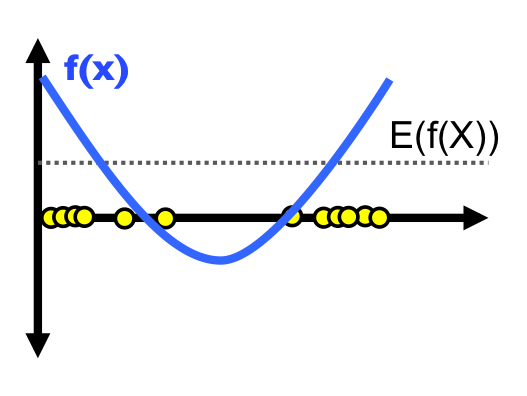
\includegraphics[width=0.6\columnwidth]{figs/update-arch3.png}
 \caption{The minimum variance estimate of an expected value of a function of a random variable $\mathbb{E}(f(X))$ is found by placing more samples (marked in yellow) on the ``spikes" of the function.\label{update-arch3}}
\end{figure}

